% !TEX root = ../main.tex
\chapter{Theory of heavy ion collisions}
  %
  % ========
  \section{The Standard Model}
  % ========
    In the 1970s, a new theory of fundamental particles and their interaction emerged.
    A new concept, which concerns the electromagnetic, weak and strong nuclear interactions between know particles.
    This theory is called \textit{The Standard Model}.
    There are seventeen named particles in the standard model, organized into the chart shown below (Fig. \ref{standard_model}).
    Fundamental particles are divided into two families: \textit{fermions} and \textit{bosons}.
     \begin{figure}[h]
       \centering
       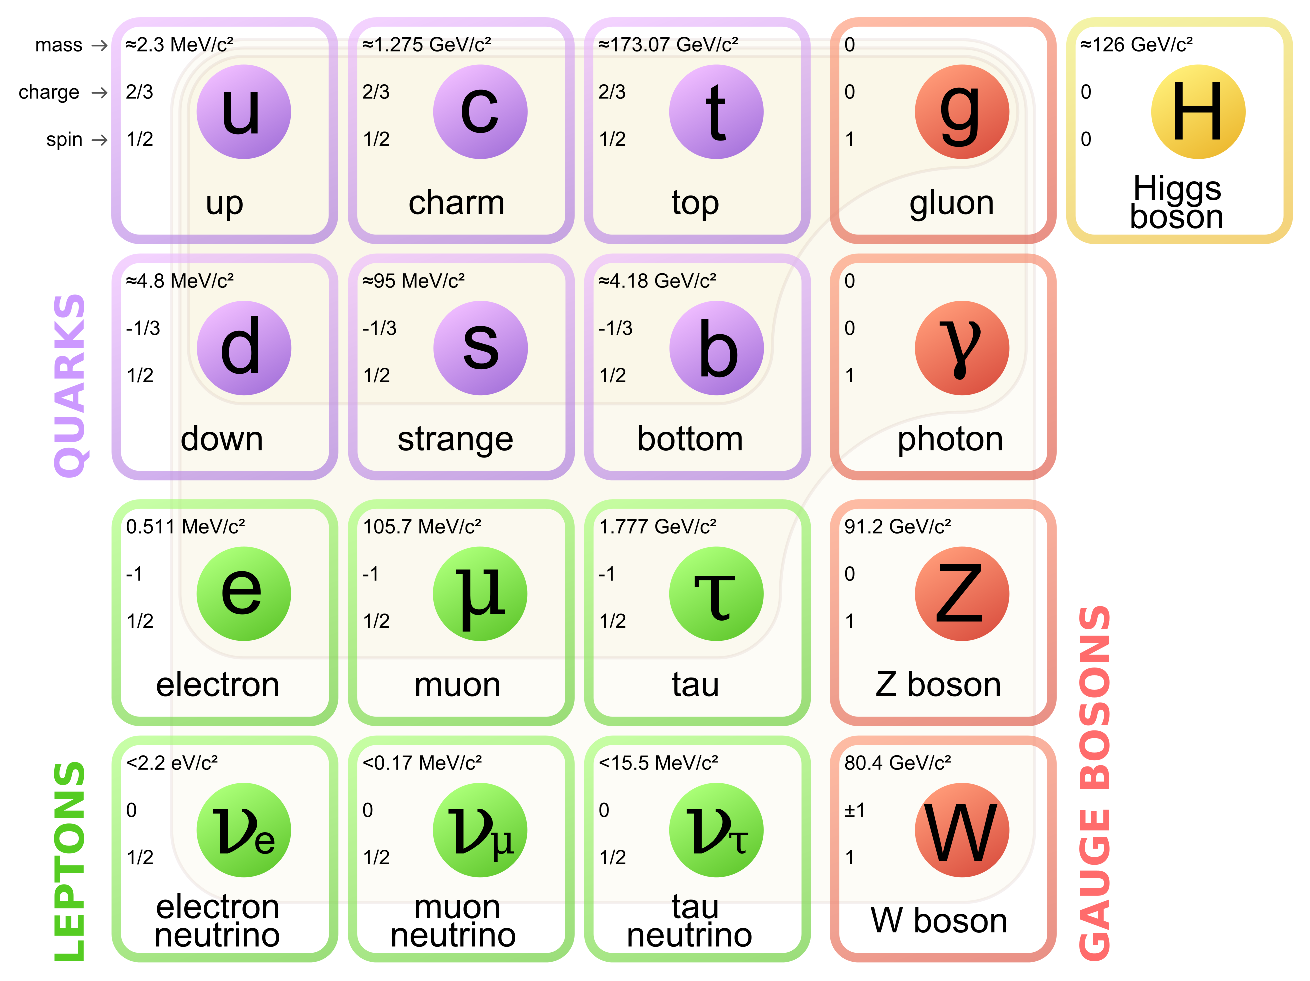
\includegraphics[width=0.9\textwidth]{standard_model}
       \caption{The Standard Model of elementary particles~\cite{sm_svg}.}
       \label{standard_model}
     \end{figure}
     
    Fermions are the building blocks of matter.
    They are divided into two groups.
    Six of them, which must bind together are called \textit{quarks}.
    Quarks are known to bind into doublets (\textit{mesons}), triplets (\textit{baryons}) and recently confirmed four-quark states.\footnote{The LHCb experiment at CERN in Geneva confirmed recently existence of $Z$(4430) - a particle consisting of four quarks~\cite{fourquark}.}
    Two of baryons, with the longest lifetimes, are forming a nucleus: a proton and a neutron.
    A proton is build from two up quarks and one down, and neutron consists of two down quarks and one up.
    A proton is found to be a stable particle (at least it has a lifetime larger than $10^{35}$ years) and a free neutron has a mean lifetime about $8.8\times10^2$ s.
    Fermions, that can exist independently are called \textit{leptons}.
    Neutrinos are a subgroup of leptons, which are only influenced by weak interaction.
    Fermions can be divided into three generations (three columns in the Figure \ref{standard_model}).
    Generation I particles can combine into hadrons with the longest life spans. 
    Generation II and III consists of unstable particles which form also unstable hadrons. 
    
    Bosons are force carriers.
    There are four fundamental forces: weak - responsible for radioactive decay, strong - coupling quarks into hadrons, electromagnetic - between charged particles and gravity - the weakest, which causes the attraction between particles with a mass.
    The Standard Model describes the first three.
    The weak force is mediated by $W^{\pm}$ and $Z^0$ bosons, electromagnetic force is carried by photons $\gamma$ and the carriers of a strong interaction are gluons \textit{g}.
    The fifth boson is a Higgs boson which is responsible for giving other particles mass. 
 
  %
  % ========
  \section{Quantum Chromodynamics}
  % ========

  % strong force bullshit
  % quark colors
  % qcd potential - confinement
  % qcd diagram
  % QGP signatures?
  Quarks interact with each other through the strong interaction.
  The mediator of this force is a \textit{gluon} - a massless and chargeless particle.
  In the quantum chromodynamics (QCD) - theory describing strong interaction - there are six types of ``charges'' (like electrical charges in the electrodynamics) called \textit{colours}.
  Some of the observed particles, like $\Delta^{-}$, $\Delta^{++}$ and $\Omega^{-}$ appeared to consist of three quarks with the same flavour (\textit{ddd}, \textit{uuu} and \textit{sss} respectively), which was in conflict with the Pauli principle.
  

  %
  % ========
  \section{Relativistic heavy ion collisions}
  % ========
%powrot do poczatkow wszechswiata
